%%%%%%%%%%%%%%%%%%%%%%%%%%%%%%%%%%%%%%%%%
% Beamer Presentation
% LaTeX Template
% Version 1.0 (10/11/12)
%
% This template has been downloaded from:
% http://www.LaTeXTemplates.com
%
% License:
% CC BY-NC-SA 3.0 (http://creativecommons.org/licenses/by-nc-sa/3.0/)
%
%%%%%%%%%%%%%%%%%%%%%%%%%%%%%%%%%%%%%%%%%

%----------------------------------------------------------------------------------------
%	PACKAGES AND THEMES
%----------------------------------------------------------------------------------------

\documentclass{beamer}

\mode<presentation> {

% The Beamer class comes with a number of default slide themes
% which change the colors and layouts of slides. Below this is a list
% of all the themes, uncomment each in turn to see what they look like.

%\usetheme{default}
%\usetheme{AnnArbor}
%\usetheme{Antibes}
%\usetheme{Bergen}
%\usetheme{Berkeley}
%\usetheme{Berlin}
%\usetheme{Boadilla}
%\usetheme{CambridgeUS}
%\usetheme{Copenhagen}
%\usetheme{Darmstadt}
%\usetheme{Dresden}
%\usetheme{Frankfurt}
%\usetheme{Goettingen}
%\usetheme{Hannover}
%\usetheme{Ilmenau}
%\usetheme{JuanLesPins}
%\usetheme{Luebeck}
\usetheme{Madrid}
%\usetheme{Malmoe}
%\usetheme{Marburg}
%\usetheme{Montpellier}
%\usetheme{PaloAlto}
%\usetheme{Pittsburgh}
%\usetheme{Rochester}
%\usetheme{Singapore}
%\usetheme{Szeged}
%\usetheme{Warsaw}

% As well as themes, the Beamer class has a number of color themes
% for any slide theme. Uncomment each of these in turn to see how it
% changes the colors of your current slide theme.

%\usecolortheme{albatross}
%\usecolortheme{beaver}
%\usecolortheme{beetle}
%\usecolortheme{crane}
%\usecolortheme{dolphin}
%\usecolortheme{dove}
%\usecolortheme{fly}
%\usecolortheme{lily}
%\usecolortheme{orchid}
%\usecolortheme{rose}
%\usecolortheme{seagull}
%\usecolortheme{seahorse}
%\usecolortheme{whale}
%\usecolortheme{wolverine}

%\setbeamertemplate{footline} % To remove the footer line in all slides uncomment this line
%\setbeamertemplate{footline}[page number] % To replace the footer line in all slides with a simple slide count uncomment this line

%\setbeamertemplate{navigation symbols}{} % To remove the navigation symbols from the bottom of all slides uncomment this line
}

\usepackage{graphicx} % Allows including images
\usepackage{booktabs} % Allows the use of \toprule, \midrule and \bottomrule in tables

%----------------------------------------------------------------------------------------
%	TITLE PAGE
%----------------------------------------------------------------------------------------

\title[Short title]{Efimov Physics -- The Three-Body Problem} % The short title appears at the bottom of every slide, the full title is only on the title page

\author{Kajsa-My Blomdahl} % Your name
\institute[SU] % Your institution as it will appear on the bottom of every slide, may be shorthand to save space
{
Stockholms Universitet \\ % Your institution for the title page
\medskip
\textit{kajsamy.blomdahl@fysik.su.se} % Your email address
}
\date{\today} % Date, can be changed to a custom date

\begin{document}

\begin{frame}
\titlepage % Print the title page as the first slide
\end{frame}

%----------------------------------------------------------------------------------------
%	PRESENTATION SLIDES
%----------------------------------------------------------------------------------------

\begin{frame}
\frametitle{The Peculiar Efimov Effect}
\begin{itemize}
\item Resonant 2-body forces can give rise to a series of bound energy levels in 3-particle systems.
\item The size of each Efimov state is much larger than the force-range between the individual particle pairs $\rightarrow$ quantum mechanical state.
\item When the two-body s-wave scattering length $a \rightarrow \pm\infty$ the $\#$ of bound states is infinite.
\item  $\#$ of 3-body bound states is \textit{reduced} as the two-body interaction is made more attractive.
\item Emerge irrespective of the nature of the 2-body forces and can \textit{in principle} be observed in all quantum mechanical systems. 
\end{itemize}
\end{frame}

%------------------------------------------------

\begin{frame}
\frametitle{Scattering Length}
\begin{itemize}
	\item The 2-body $s$-wave scattering length characterise the strength of the interparticle interaction. Definition:
	\begin{equation}
	a = \lim_{k \to 0} -\frac{\tan\delta_0(k)}{k}
	\end{equation}
	\item Negative scattering lengths correspond to an attractive effective interaction.
	\item Positive scattering lengths correspond to a repulsive effective interaction.
\end{itemize}
\end{frame}

\begin{frame}
\frametitle{The 2-body Problem}
\begin{block}{2-body Scattering}
	Particles with large scattering lengths in the low-energy regime have universal properties. 
\end{block}

\begin{block}{Universal Properties.. In What Sense?}
	Depend on the scattering length alone and not on the details of the short-range interaction.
\end{block}

\begin{block}{Exemple: 2B Binding Energy For 2 Identical Bosons}
	\begin{equation}
	E_D = \frac{\hbar^2}{2 \mu_{2b} a^2}.
	\end{equation}
\end{block}
\end{frame}

\begin{frame}
\frametitle{Universality in 3-Body Systems}
\begin{figure}
	\centering
	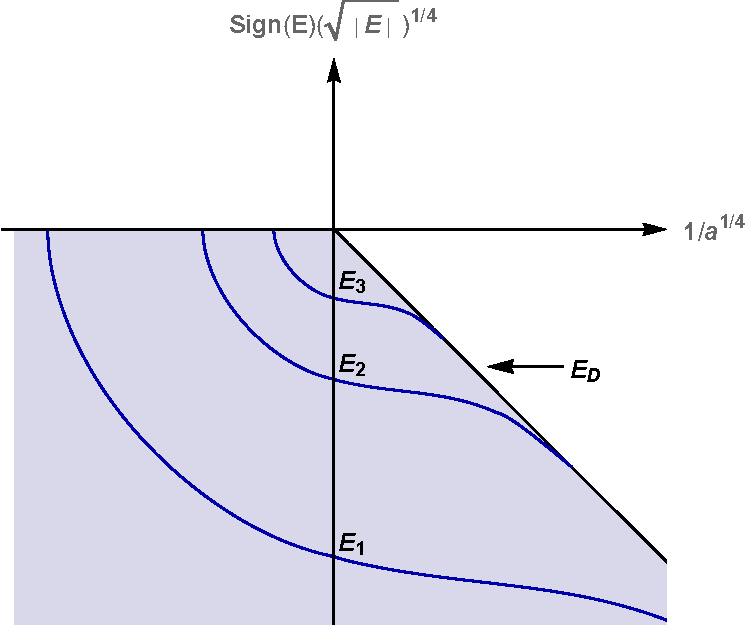
\includegraphics[width=0.5\linewidth]{efimov}
	\caption{The energies of the three first Efimov states are plotted as functions of the inverse scattering length $a$. Three different regions can be identified in the figure.	The energy levels scale geometrically: $\frac{E_T^{n+1}}{E_T^{n}} = e^{2\pi/s_0} \approx 515$, for identical bosons ($s_0 \simeq 1.00624$ for $J=0^+$ states).}
\end{figure} 
\end{frame}

\begin{frame}
\frametitle{Cause}
\centerline{Emergent Attractive 3-Body Potentials}
\end{frame}

\begin{frame}
\frametitle{3-Particles, What Is The Problem?!}
\begin{block}{Apparently simple, However}
	\begin{itemize}
	\item The configuration space for the 3BP is 6D after separating out the center of mass motion.
	\item 3 additional constants of motion can be provided by conservation of the total angular momentum.
	\item This leaves a three dimensional Schr{\"o}dinger equation in the quantum case.
	\end{itemize}
\end{block}
\end{frame}

\begin{frame}
\frametitle{Solving The 3-body Problem: Step 1, Jacobi Coordinates}
\begin{figure}
\centering
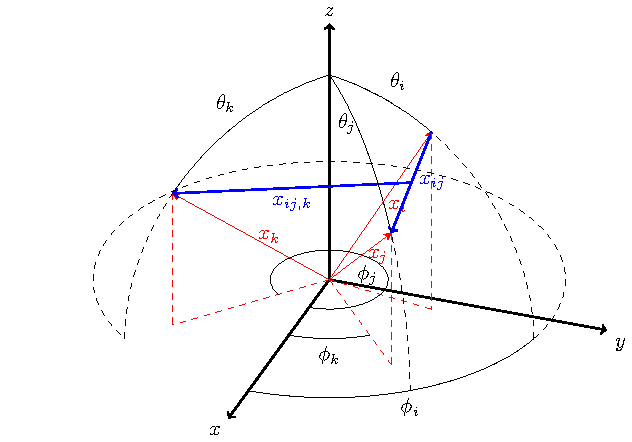
\includegraphics[width=0.7\linewidth]{img01.pdf}
\caption{Spatial positions of three particles.}
\end{figure}
\end{frame}

\begin{frame}
\frametitle{Solving The 3-body Problem: Step 2, Hyperspherical Coordinates}
\begin{itemize}
	\item Separate internal and external coordinates
	\item Internal coordinates: 1 hyperradius: controls the size 
	\item Internal coordinates: 2 hyperangles: shape and particle permutations
\end{itemize}
\end{frame}

\begin{frame}
\frametitle{Solving The 3-body Problem: Step 3, Adiabatic Representation}
The Schr{\"o}dinger equation in hyperspherical coordinates
\begin{equation}
\bigg(-\frac{1}{2 \mu}\frac{\partial^2}{\partial \rho^2} + \frac{ \Lambda^2 + \frac{15}{4}}{2 \mu \rho^{2}}+ V(\rho,\Omega)\bigg)\psi(\rho,\Omega) = E\psi(\rho,\Omega).
\end{equation}

\begin{itemize}
\item Treat the hyperradius as a parameter! 

\item $\rightarrow$ 3-body Born-Oppenheimer-like potential
\end{itemize}
\begin{equation}
H_{ad}\Phi_{\nu}{(\rho;\Omega)} = U_{\nu}{(\rho)}\Phi_{\nu}(\rho;\Omega)
\end{equation}
\end{frame}

%------------------------------------

\begin{frame}
\frametitle{Solving The 3-body Problem: Step 4, 3-Body Energies}
The total wave function, 

\begin{equation}\label{wave}
\psi_{n}(\rho,\Omega) = \sum_{\nu=0}^{\infty} F_{n\nu}(\rho)\Phi_{\nu}(\rho;\Omega),
\end{equation}
can in this way be represented in terms of adiabatic states, which, in principle, yields an exact representation of the three-body Schr{\"o}dinger equation if all couplings are included.
\end{frame}

\begin{frame}
\frametitle{Solving The 3-body Problem: Step 4, Continued}
\begin{align}\label{fullhamiltonian}
\bigg(-\frac{1}{2 \mu}\frac{\partial^2}{ \partial \rho^2} + U_{\mu}(\rho) - \frac{1}{2\mu}Q_{\mu\mu}(\rho) \bigg)F_{n\mu}(\rho)&\nonumber\\ -\frac{1}{2\mu}\bigg(\sum_{\nu\neq\mu}2P_{\mu\nu}(\rho)\frac{\partial}{\partial\rho} + Q_{\mu\nu}(\rho) \bigg)F_{n\nu}(\rho)& = E_nF_{n\mu}(\rho).
\end{align}
\end{frame}

\begin{frame}
\frametitle{Emergent Attractive and Repulsive Potentials}
In the adiabatic approximation the effective potentials are defined as 

\begin{equation}
W_{\nu}(\rho) = U_{\nu}(\rho)-\frac{1}{2\mu}Q_{\nu \nu}(\rho) = U_{\nu}(\rho)-\frac{1}{2\mu}P_{\nu \nu}^2(\rho).
\end{equation} 
These potentials are used for determining the single channel solutions of \eqref{fullhamiltonian}. 
\end{frame}

\begin{frame}
\frametitle{Effective Potentials in the Asymptotic Limit}
3 free atoms $a<0$:

\begin{equation}
W_{\nu}(\rho)  \xrightarrow{ \rho \to \infty} \frac{\lambda(\lambda+4)+\frac{15}{4}}{2\mu \rho^2}.
\end{equation}

Atom-dimer configurations $a>0$:

\begin{equation}
W_{\nu}(\rho)  \xrightarrow{ \rho \to \infty} E_{2b} +\frac{l(l+1)}{2\mu \rho^2}.
\end{equation} 
\end{frame}

\begin{frame}
\frametitle{Effective Potentials in the Intermediate Region}
Efimov physics comes into play when $r_0 \ll \rho \ll |a|$! As the scattering length grows in magnitude for $a>0$ and $a<0$ the lowest effective potential will converge to the Efimov potential 

\begin{equation}\label{eq:efimov_channel}
W_{\nu}(\rho) = -\frac{s_0^2+\frac{1}{4}}{2\mu \rho^2},
\end{equation} 
in which $s_0 \simeq 1.00624$.
\end{frame}

\begin{frame}
\frametitle{Scattering Model}
\begin{block}{3-body Masses}
	\begin{equation}
	m = m(Rubidium-87)
	\end{equation}
\end{block}

\begin{block}{Assuming the Potential Can Be Written As a Sum of 2-B Interactions}
 \begin{equation}
V(\rho,\theta,\psi) = v(r_{12}) + v(r_{23}) + v(r_{31})
\end{equation} 
\end{block}

\begin{block}{The 2-body Model Potential}
	\begin{equation}
	v(r) = d\cosh^{-2}{(r/r_0)}
	\end{equation}
\end{block}
\end{frame}

\begin{frame}
\begin{figure}
	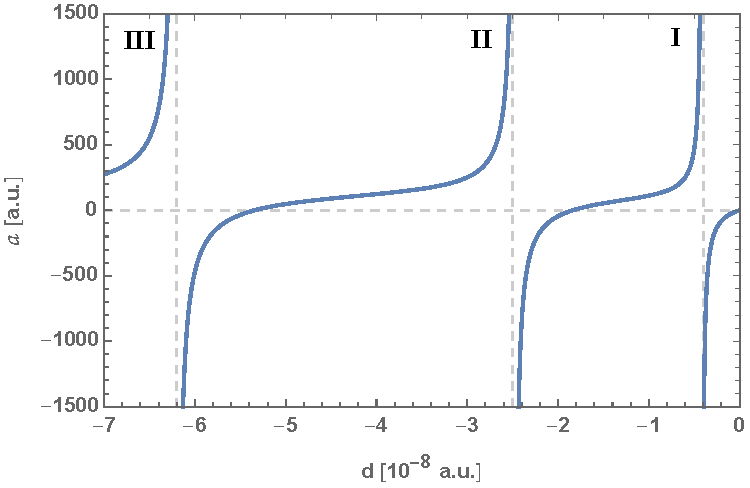
\includegraphics[width=0.7\linewidth]{scatteringlength.pdf}
\end{figure}
\end{frame}

\begin{frame}
\frametitle{$a>0$}
\begin{figure}
	\begin{figure}
		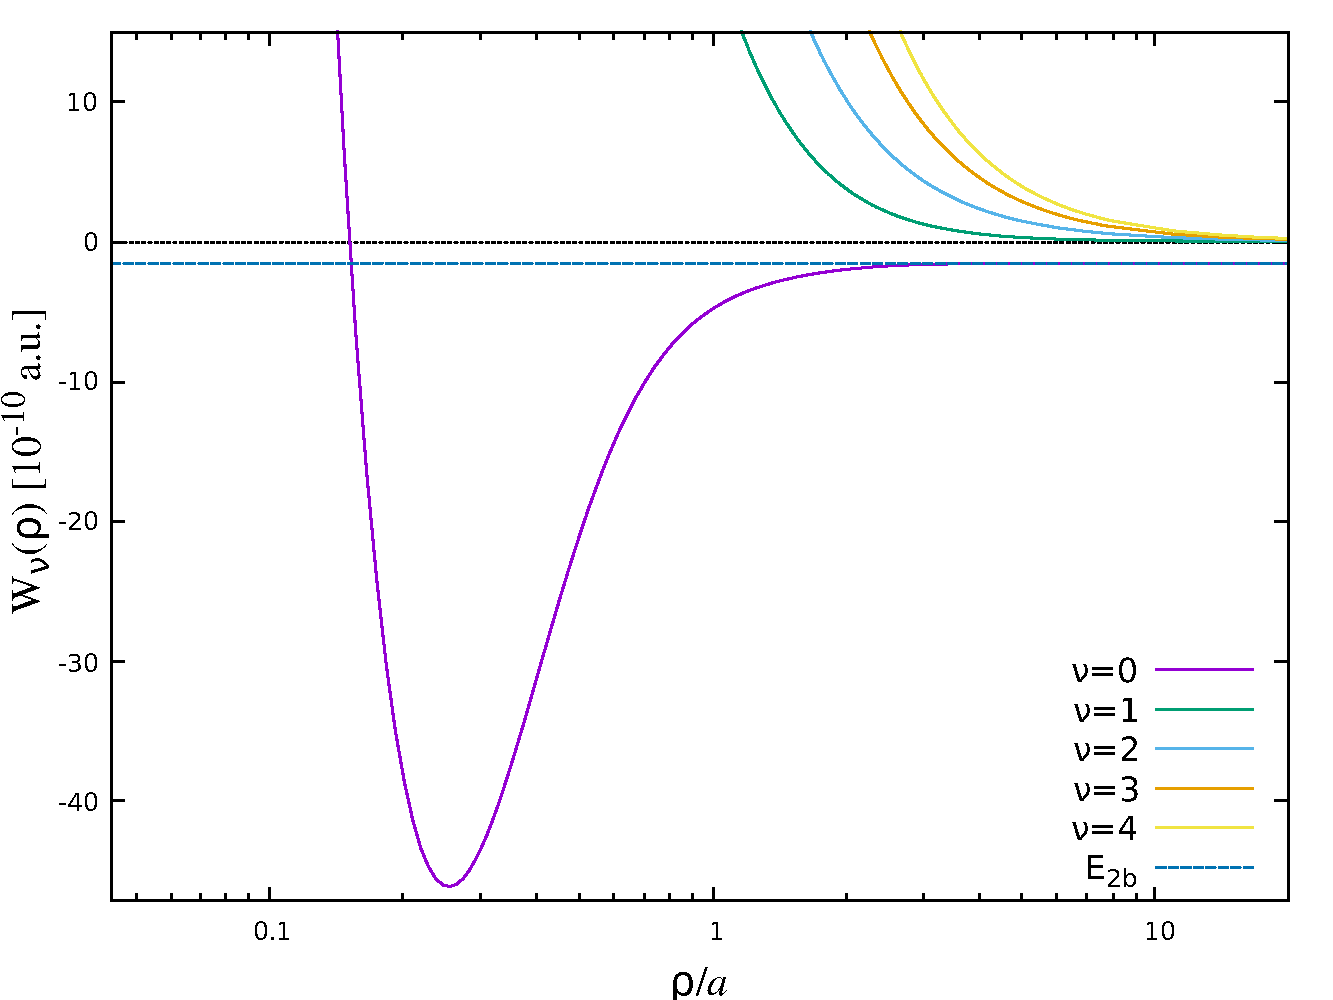
\includegraphics[width=0.8\linewidth]{Wpos.pdf}
	\end{figure}
\end{figure}
\end{frame}

\begin{frame}
\frametitle{$a<0$}
\begin{figure}
	\begin{figure}
		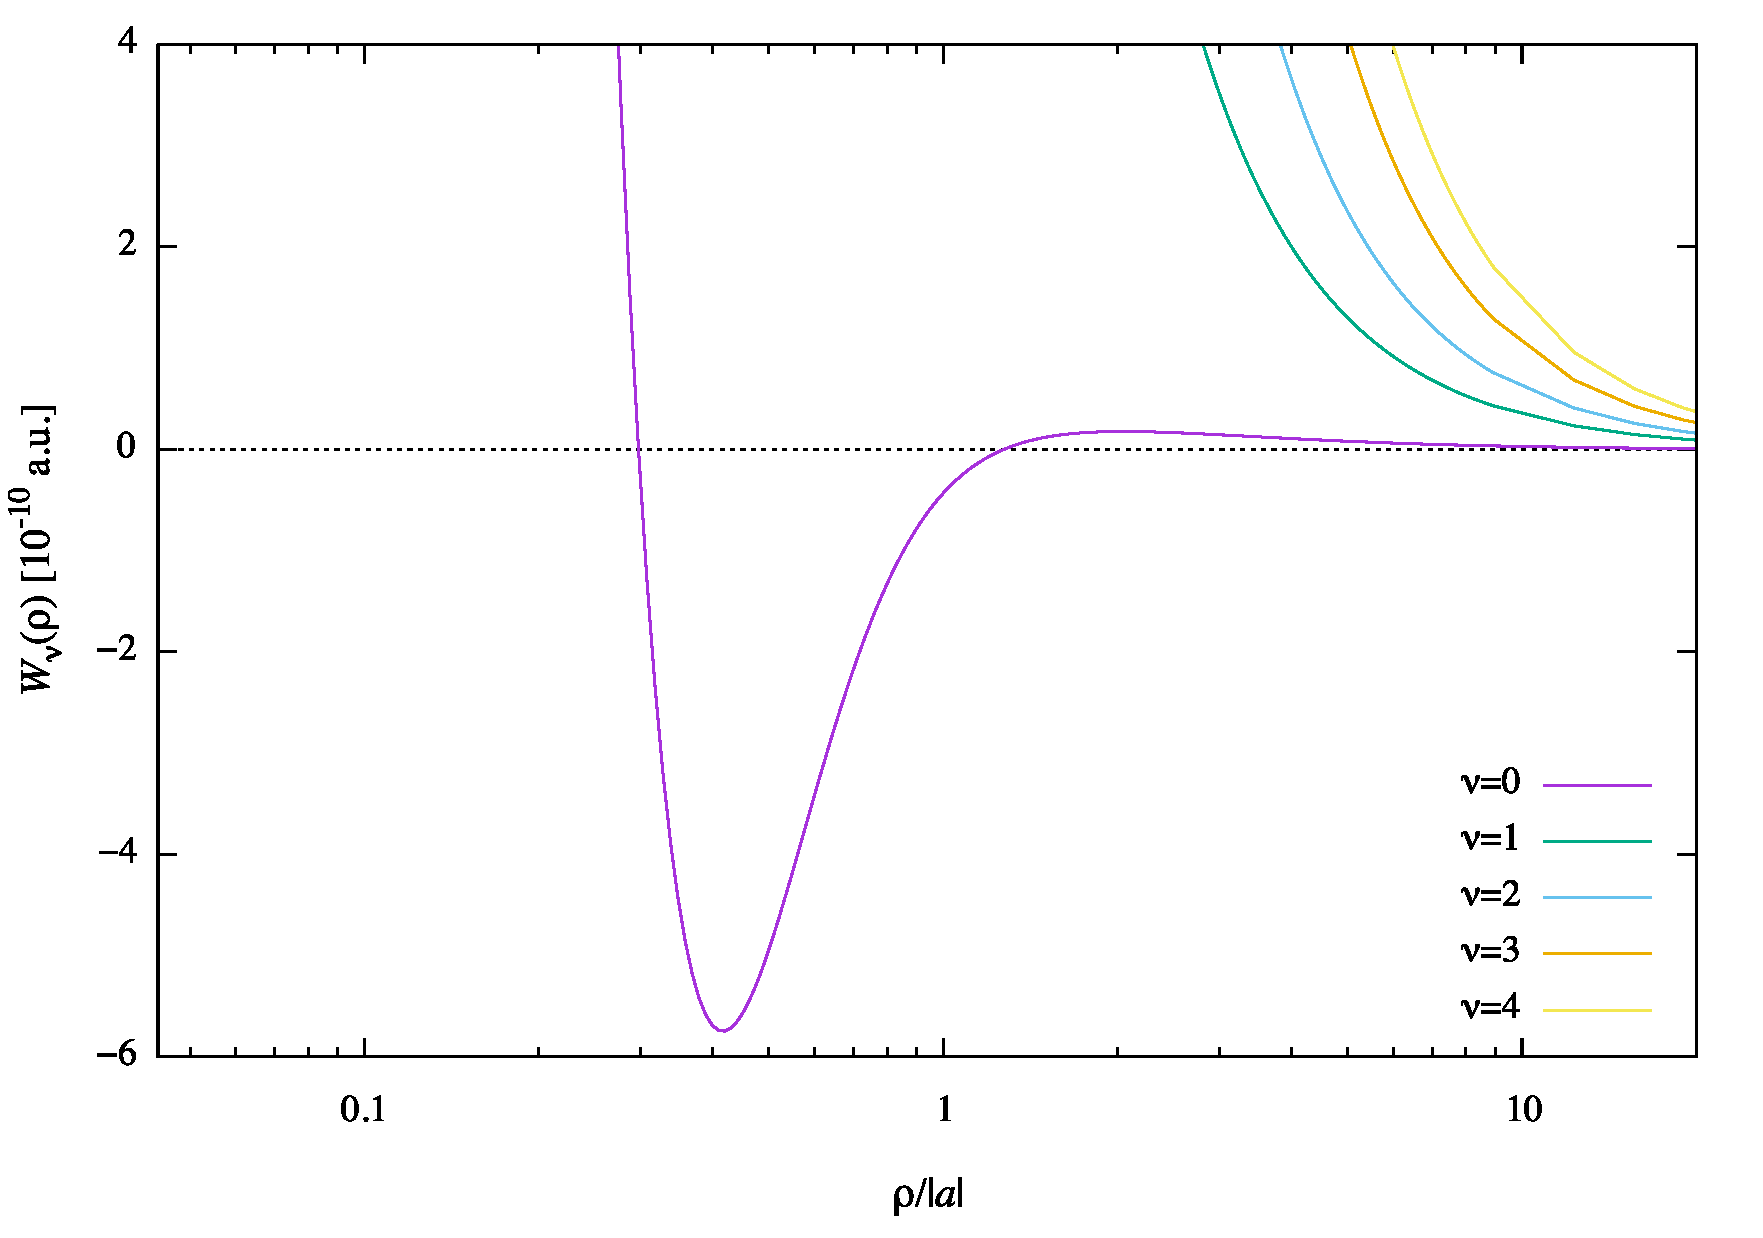
\includegraphics[width=0.8\linewidth]{Wneg.pdf}
	\end{figure}
\end{figure}
\end{frame}

%------------------------------------------------

\begin{frame}
\frametitle{Efimov Potentials}
We expect that the lowest effective potential curve will converge towards

\begin{equation}
W_{\nu}(\rho) = -\frac{s_0^2+\frac{1}{4}}{2\mu \rho^2},
\end{equation} 
for $|a| \rightarrow \infty$. This behaviour should be evident if the potentials are multiplied by $2 \mu \rho^2$ and plotted as 

\begin{equation}\label{eq:lambda}
\xi(\rho) = 2 \mu \rho^2 W_{\nu}(\rho) + \frac{1}{4},
\end{equation}
since these curves should approach the universal value $-s_0^2 (\simeq -1.0125$ for $J=0^+$ states).
\end{frame}


\begin{frame}
\frametitle{$a \rightarrow \pm \infty$, $-s_0^2 (\simeq -1.0125$ for $J=0^+$ states)}
\begin{figure}
	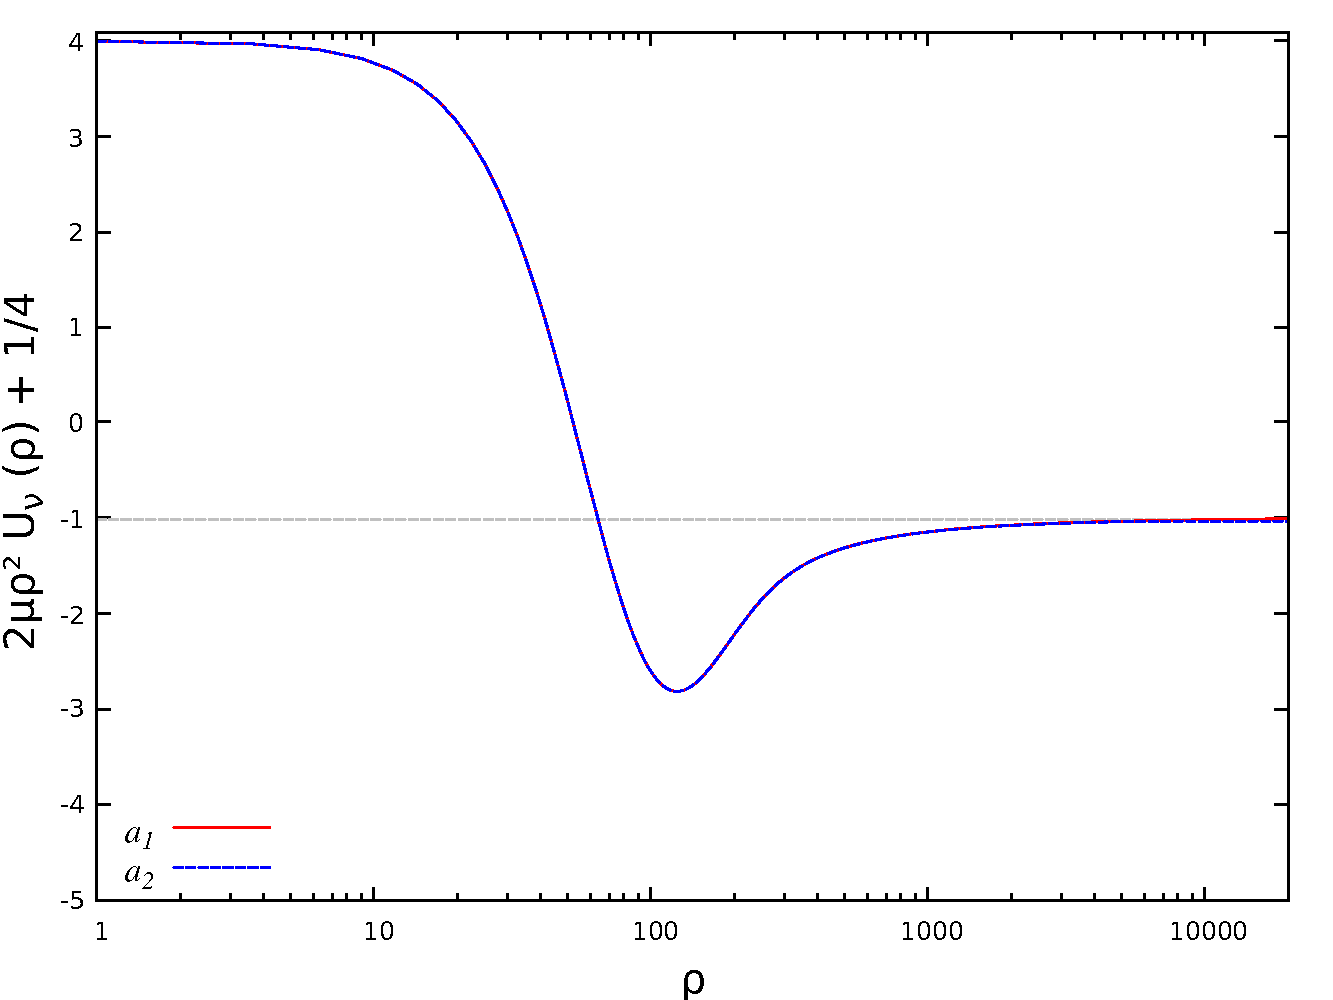
\includegraphics[width=0.8\linewidth]{infty.pdf}
\end{figure}
\end{frame}

\begin{frame}
\frametitle{$a >0$}
\begin{figure}
	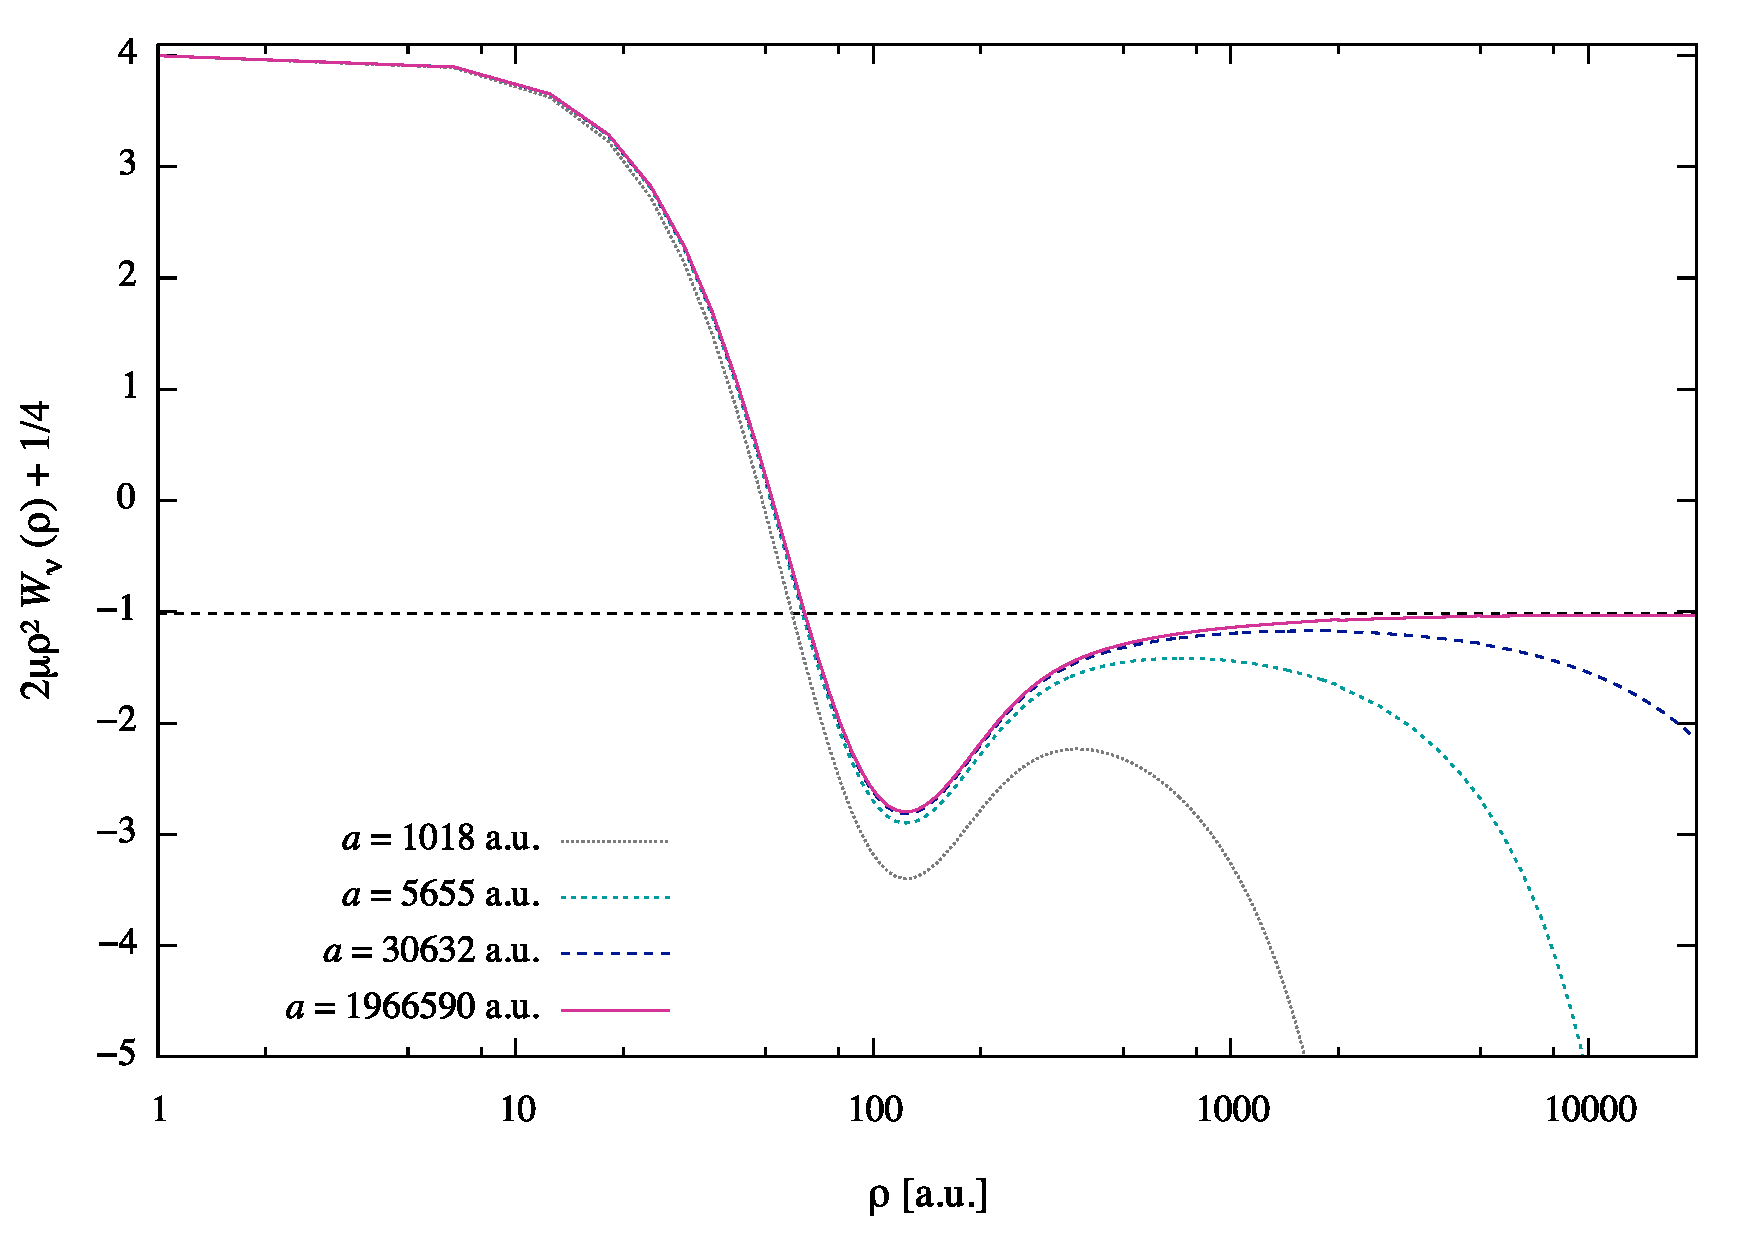
\includegraphics[width=0.8\linewidth]{finite_positive_a.pdf}
\end{figure}
\end{frame}

\begin{frame}
\frametitle{$a<0$}
\begin{figure}
	\begin{figure}
		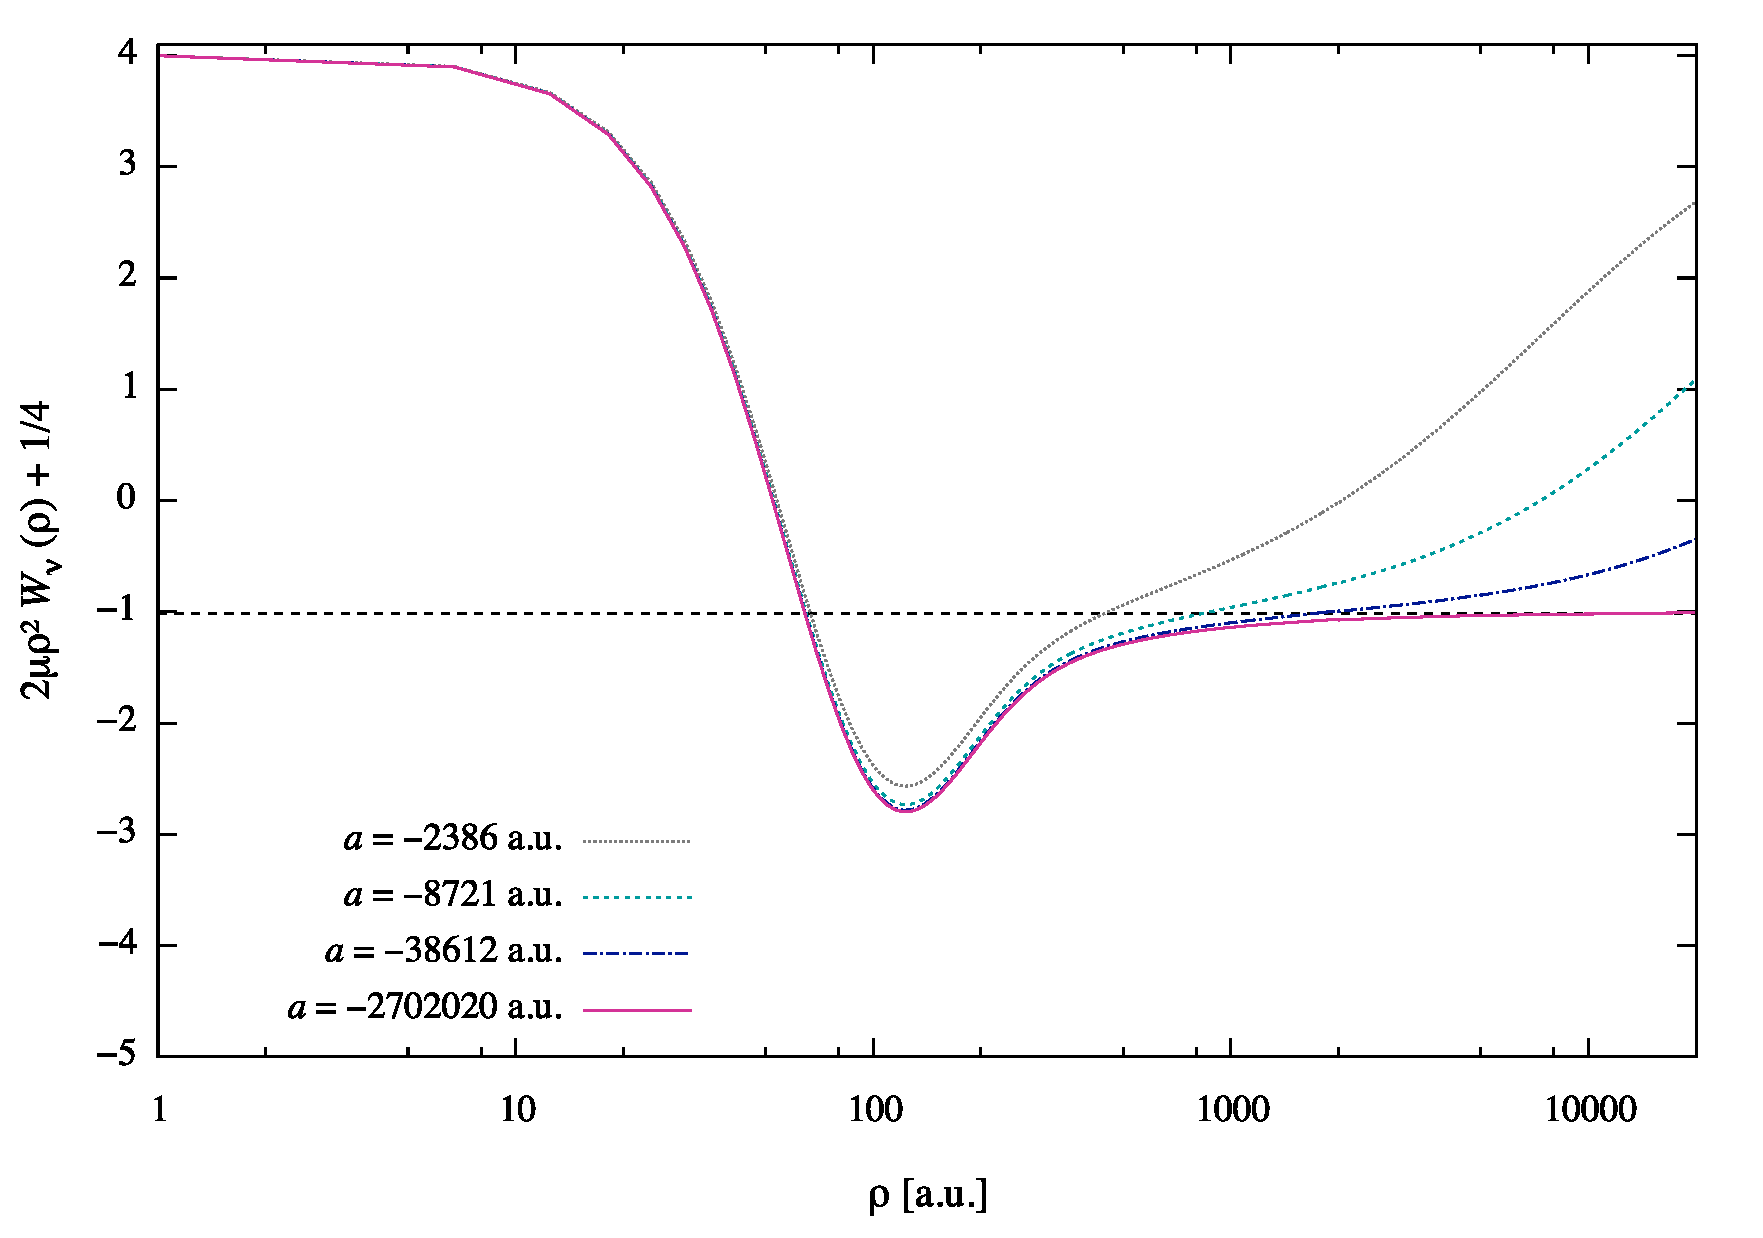
\includegraphics[width=0.8\linewidth]{finite_negative_a.pdf}
	\end{figure}
\end{figure}
\end{frame}

\begin{frame}
\frametitle{Comparison With the Adiabatic Potential From Solving Faddeev's Equation}
For $\rho \gg r_0$ the adiabatic potentials $\nu_n$ (which correspond to $ \xi(\rho)$) can be determined analytically through the transcendental equation

\begin{equation}\label{eq:transcendental}
\sqrt{\nu_n} \cos{\bigg(\sqrt{\nu_n} \frac{\pi}{2}\bigg)} - \frac{8}{\sqrt{3}}\sin{\bigg(\sqrt{\nu_n} \frac{\pi}{6}\bigg)} = \sqrt{2}\frac{\rho}{a}\sin{\bigg(\sqrt{\nu_n} \frac{\pi}{2}\bigg)}, 
\end{equation}
for different scattering lengths $a$.
\end{frame}

\begin{frame}
\frametitle{$a=-2386$ a.u.}
	\begin{figure}
		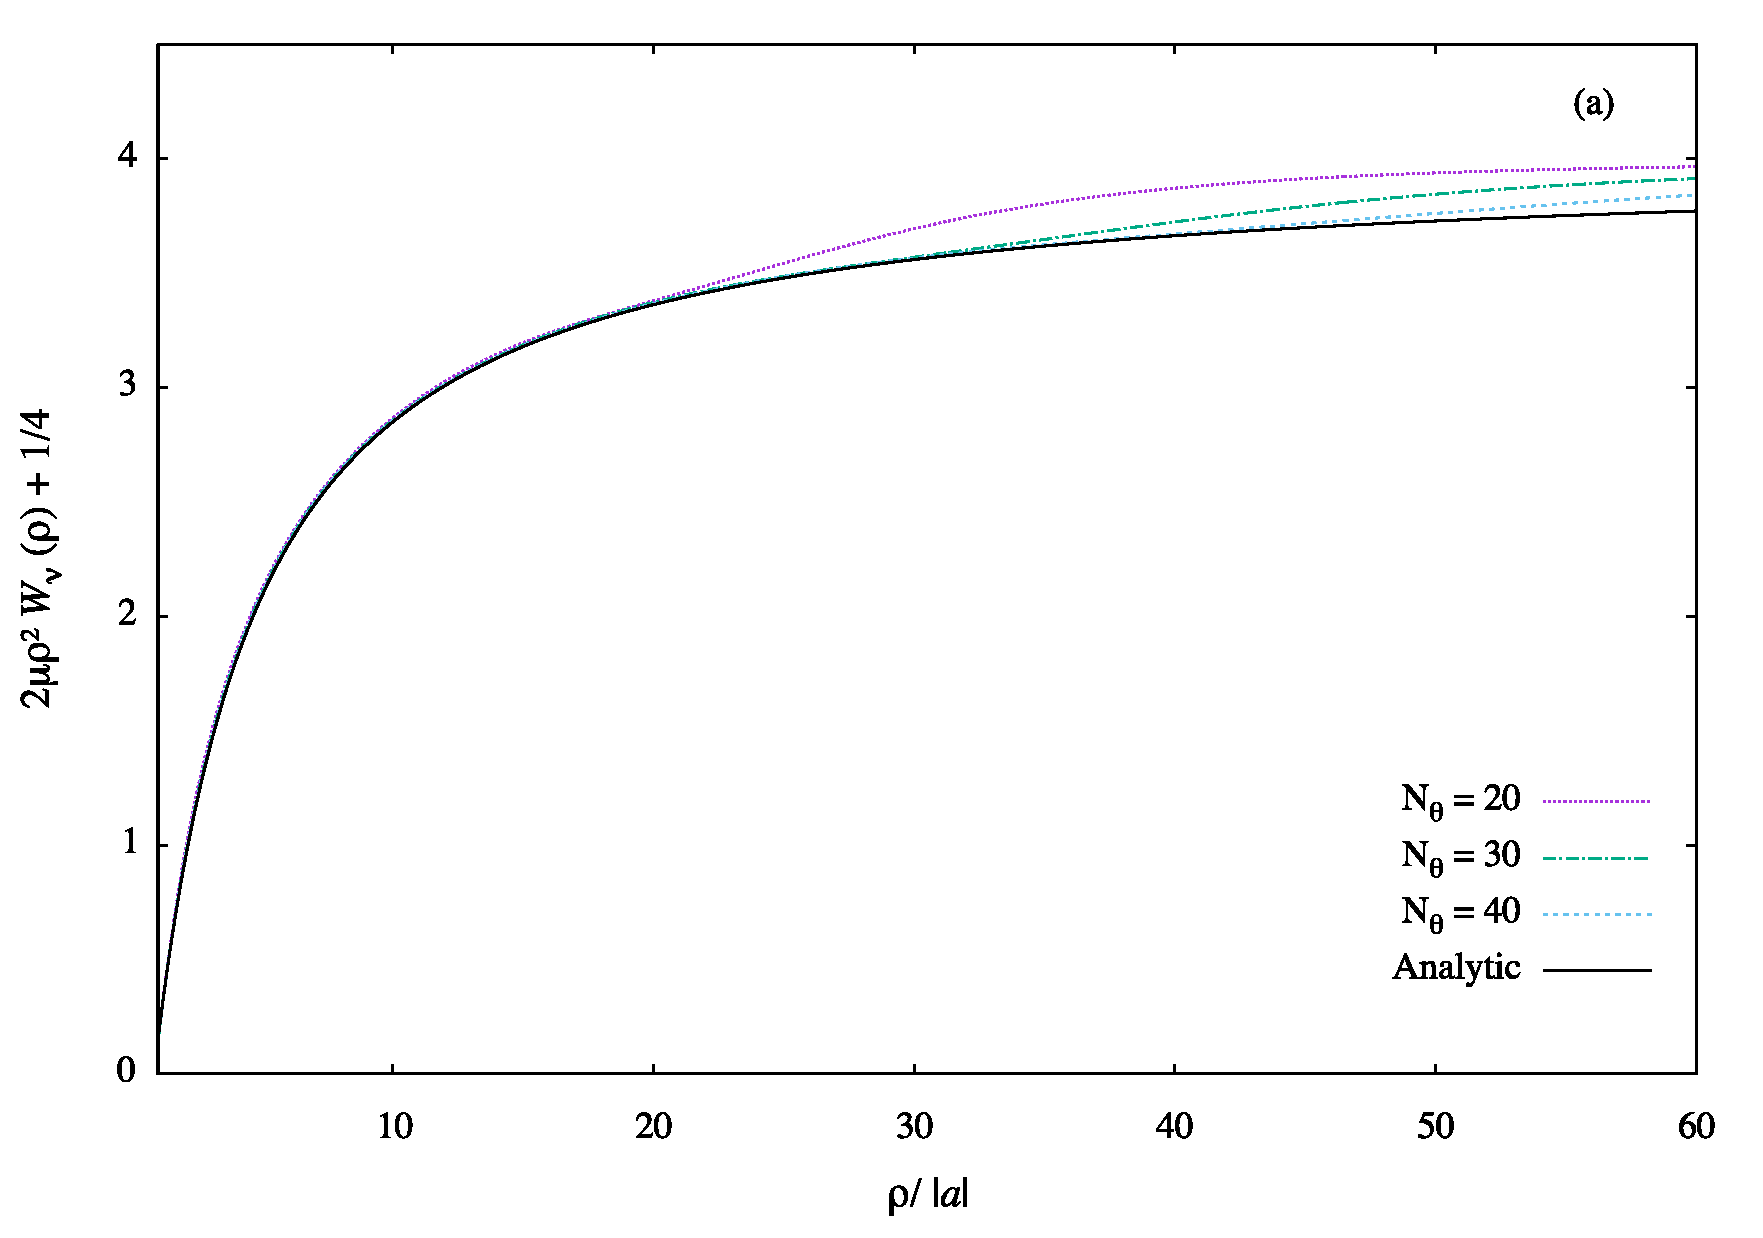
\includegraphics[width=0.8\linewidth]{convergence2.pdf}
	\end{figure}
\end{frame}

\begin{frame}
\frametitle{$a=-8721$ a.u.}
\begin{figure}
	\begin{figure}
		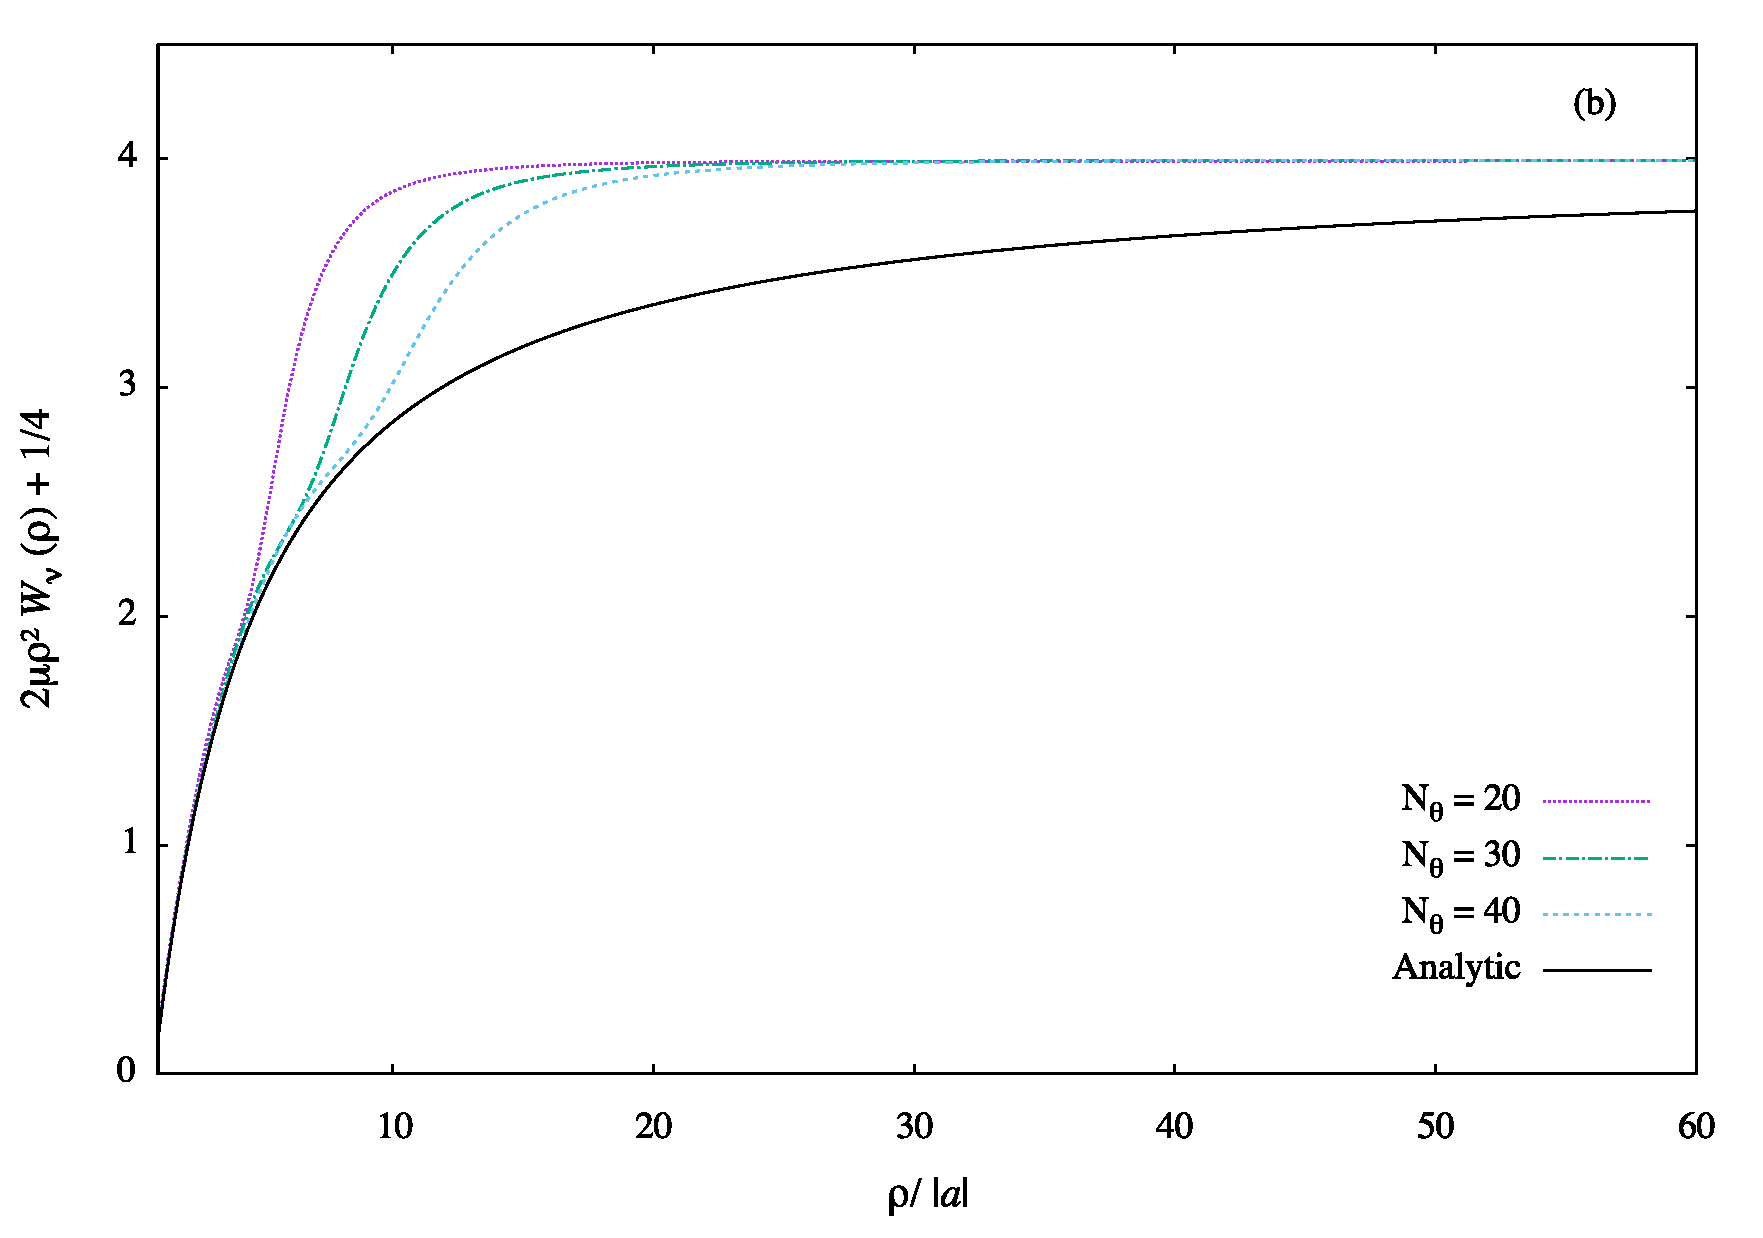
\includegraphics[width=0.8\linewidth]{convergence8.pdf}
	\end{figure}
\end{figure}
\end{frame}


%----------------------------------------------------------------------------------------

\end{document} 